\chapter{Introduction}
From 2D, to 3D and now to \acs{bim}. The evolution of the \ac{aec} industry has been a long and complex one. The introduction of 3D modeling was the first major step in the industry's evolution, as it allowed for more accurate representations of buildings. No longer solely relying on 2D drawings, a 3D model of a building can be used to create various representations, from a simple 2D floor plan to a full 3D model. Following the adoption of 3D modeling, the implementation of \ac{bim} emerged as another significant milestone. \ac{bim} adds an extra layer of information on top of the 3D model. As the digital representation of a building's physical and functional characteristics, BIM serves as a repository for semantics originating from various applications throughout the design and construction processes, including cost estimation, energy analysis, and production planning.\\
-> needs refs to support point (about infustries in AEC)

\label{sec:intro}
However, as mentioned in \cite{Werbrouck2018}, the next challenge for the \ac{aec} industry is related to the ecosystem of current \ac{bim} softwares, which remains closed off to other disciplines. This data management challenge is currently being adressed by the \ac{lbd-cg} and other research entities, such as the University of Ghent, through the use of Web of Data technologies \footcite{ldbimGroup}. This emerging milestone will be discussed in this thesis under the term \ac{ldbim}.

\subsubsection*{Proposal}
Each of these evolutions has brought, and will continue to bring, a significant amount of data together. This volume is expected to grow exponentially in the future as the industry shifts towards a more digital approach and opens up to other stakeholders. The data graphs will not only expand in terms of semantics but also in geometry. This makes visual querying, or simply put, 3D exploration of models, an increasingly difficult task. Especially when looking at newer devices used in the industry such as mobile phones, and tablets, which are becoming more and more powerful, but still have limited computational resources in comparison to office computers.

To bring this volume of geometric data in perspective, Table \ref{tab:sizeModels} shows the size of the test-models used in \cite{Johansson2015} , a study from 2015 on the performance of \ac{bim} viewers for large models with the following description:

\enquote{
	Although the Hotel model contains some structural elements they are primarily architectural models. As such, no Mechanical, Electrical or Plumbing (MEP) data is present. However, all models except the Hospital contain furniture and other interior equipment.
} \parencite{Johansson2015}

\begin{table}[h]
	\centering
	\begin{tabular}{@{}lrrr@{}}
		\toprule
		Model         & \multicolumn{1}{l}{\# of  triangles} & \multicolumn{1}{l}{\# of objects} & \multicolumn{1}{l}{\# of geometry batches} \\ \midrule
		Library       & 3 685 748                            & 7318                              & 11 195                                     \\
		Student House & 11 737 251                           & 17 674                            & 33 455                                     \\
		Hospital      & 2 344 968                            & 18627                             & 22 265                                     \\
		Hotel         & 7 200 901                            & 41 893                            & 62 624                                     \\ \bottomrule
	\end{tabular}
	\caption{Size of test-models in \cite{Johansson2015}}
	\label{tab:sizeModels}
\end{table}

These models demonstrate how basic \ac{bim} models can already contain a significant amount of data. \ac{ldbim} will not only bring together new stakeholders but also have the capability to keep track of multiple geometry versions for each object, should they occur. Therefore, this thesis proposes a new approach to the visual querying of \ac{ldbim} models, wherein viewers will not have to load the entire model into memory. Instead, after filtering at the source, only the geometry needed for the visual tasks at hand will be loaded, while maintaining the original link to each resource for further processing and use cases. This filtering step is commonly referred to as culling in the computer graphics industry and is illustrated in Figures \ref{fig:firstIdea} and \ref{fig:cullingPrinciple}.

\begin{figure}[h]
	\centering
	% made with Mathcha.io
\tikzset{every picture/.style={line width=0.75pt}} %set default line width to 0.75pt        

\begin{tikzpicture}[x=0.75pt,y=0.75pt,yscale=-1,xscale=1]
    %uncomment if require: \path (0,215); %set diagram left start at 0, and has height of 215

    %Flowchart: Magnetic Disk [id:dp6284829251226534] 
    \draw   (513.6,38.45) -- (513.6,83.95) .. controls (513.6,90.72) and (491.89,96.2) .. (465.1,96.2) .. controls (438.31,96.2) and (416.6,90.72) .. (416.6,83.95) -- (416.6,38.45)(513.6,38.45) .. controls (513.6,45.22) and (491.89,50.7) .. (465.1,50.7) .. controls (438.31,50.7) and (416.6,45.22) .. (416.6,38.45) .. controls (416.6,31.68) and (438.31,26.2) .. (465.1,26.2) .. controls (491.89,26.2) and (513.6,31.68) .. (513.6,38.45) -- cycle ;
    %Shape: Ellipse [id:dp6455225472033841] 
    \draw   (325.26,24.56) .. controls (325.26,19.17) and (329.51,14.8) .. (334.75,14.8) .. controls (339.99,14.8) and (344.23,19.17) .. (344.23,24.56) .. controls (344.23,29.95) and (339.99,34.32) .. (334.75,34.32) .. controls (329.51,34.32) and (325.26,29.95) .. (325.26,24.56) -- cycle ;
    %Straight Lines [id:da5518509163242133] 
    \draw    (334.75,34.32) -- (334.75,64.57) ;
    %Straight Lines [id:da9145784090055042] 
    \draw    (334.75,64.57) -- (347.8,78) ;
    %Straight Lines [id:da22424775934882302] 
    \draw    (334.75,64.57) -- (322.05,77.63) ;
    %Straight Lines [id:da8489215579129423] 
    \draw    (323.45,45.1) -- (345.68,45.1) ;

    %Straight Lines [id:da5548656651310764] 
    \draw  [dash pattern={on 3pt off 2.25pt}]  (335.2,105) -- (335.2,205.4) ;
    %Straight Lines [id:da5101755880224319] 
    \draw  [dash pattern={on 3pt off 2.25pt}]  (465.6,105) -- (465.6,204.2) ;
    %Straight Lines [id:da5195810822633473] 
    \draw    (339.8,130.4) -- (460.2,130.4) ;
    \draw [shift={(462.2,130.4)}, rotate = 180] [color={rgb, 255:red, 0; green, 0; blue, 0 }  ][line width=0.75]    (10.93,-3.29) .. controls (6.95,-1.4) and (3.31,-0.3) .. (0,0) .. controls (3.31,0.3) and (6.95,1.4) .. (10.93,3.29)   ;
    %Straight Lines [id:da6802623628359596] 
    \draw    (342.2,182) -- (462.6,182) ;
    \draw [shift={(340.2,182)}, rotate = 0] [color={rgb, 255:red, 0; green, 0; blue, 0 }  ][line width=0.75]    (10.93,-3.29) .. controls (6.95,-1.4) and (3.31,-0.3) .. (0,0) .. controls (3.31,0.3) and (6.95,1.4) .. (10.93,3.29)   ;
    %Curve Lines [id:da9923382034402601] 
    \draw [color=ugentblue  ,draw opacity=1 ]   (471,150.2) .. controls (506.64,136.88) and (517.58,179.73) .. (472,157.69) ;
    \draw [shift={(470.6,157)}, rotate = 26.57] [color=ugentblue  ,draw opacity=1 ][line width=0.75]    (10.93,-3.29) .. controls (6.95,-1.4) and (3.31,-0.3) .. (0,0) .. controls (3.31,0.3) and (6.95,1.4) .. (10.93,3.29)   ;
    %Shape: Rectangle [id:dp4685611128558902] 
    \draw  [draw opacity=0] (244.2,8.1) -- (555.4,8.1) -- (555.4,212.2) -- (244.2,212.2) -- cycle ;

    % Text Node
    \draw (432.6,61.2) node [anchor=north west][inner sep=0.75pt]   [align=left] {Database};
    % Text Node
    \draw (317.2,83) node [anchor=north west][inner sep=0.75pt]   [align=left] {HHD};
    % Text Node
    \draw  [draw opacity=0][fill={rgb, 255:red, 255; green, 255; blue, 255 }  ,fill opacity=1 ]  (371,116) -- (429,116) -- (429,141) -- (371,141) -- cycle  ;
    \draw (374,120) node [anchor=north west][inner sep=0.75pt]   [align=left] {request};
    % Text Node
    \draw  [draw opacity=0][fill={rgb, 255:red, 255; green, 255; blue, 255 }  ,fill opacity=1 ]  (371.4,167.6) -- (429.4,167.6) -- (429.4,192.6) -- (371.4,192.6) -- cycle  ;
    \draw (374.4,171.6) node [anchor=north west][inner sep=0.75pt]   [align=left] {request};
    % Text Node
    \draw (506.8,145.8) node [anchor=north west][inner sep=0.75pt]  [color=ugentblue  ,opacity=1 ] [align=left] {culling};


\end{tikzpicture}

	\caption{Sequence diagram - basic concept}
	\label{fig:firstIdea}
\end{figure}

Figure \ref{fig:firstIdea} illustrates the basic idea of this thesis, presenting an extra step in the communication between a user, represented here by a \ac{hhd}, and a database storing the model. An \ac{hhd} has been chosen to exemplify a low-powered device used in the field, which requires a lightweight 3D viewer to visualize and explore the digital twin of the building. The \ac{hhd} is assumed to have no knowledge of the \ac{ldbim} model and only receives the geometry that needs to be displayed from the database. On the other hand, the database is assumed to possess, or have access to, all the knowledge of the model and the necessary semantics to perform the culling.

\begin{figure}[h]
	\centering
	

% Gradient Info

\tikzset {_lnfkxmyfs/.code = {\pgfsetadditionalshadetransform{ \pgftransformshift{\pgfpoint{0 bp } { 0 bp }  }  \pgftransformrotate{0 }  \pgftransformscale{2 }  }}}
\pgfdeclarehorizontalshading{_mlgazkjgj}{150bp}{rgb(0bp)=(0,0,0);
    rgb(53.839285714285715bp)=(0,0,0);
    rgb(62.5bp)=(0,0,0);
    rgb(100bp)=(0,0,0)}
\tikzset{_ss8aeyqug/.code = {\pgfsetadditionalshadetransform{\pgftransformshift{\pgfpoint{0 bp } { 0 bp }  }  \pgftransformrotate{0 }  \pgftransformscale{2 } }}}
\pgfdeclarehorizontalshading{_jjajrhv3n} {150bp} {color(0bp)=(transparent!90);
    color(53.839285714285715bp)=(transparent!90);
    color(62.5bp)=(transparent!100);
    color(100bp)=(transparent!100) }
\pgfdeclarefading{_vtdml7b05}{\tikz \fill[shading=_jjajrhv3n,_ss8aeyqug] (0,0) rectangle (50bp,50bp); }
\tikzset{every picture/.style={line width=0.75pt}} %set default line width to 0.75pt        

\begin{tikzpicture}[x=0.75pt,y=0.75pt,yscale=-1,xscale=1]
    %uncomment if require: \path (0,300); %set diagram left start at 0, and has height of 300

    %Shape: Polygon [id:ds5156023997500794] 
    \draw  [draw opacity=0][shading=_mlgazkjgj,_lnfkxmyfs,path fading= _vtdml7b05 ,fading transform={xshift=2}] (290.57,117.14) -- (527,29.25) -- (527,281.75) -- (338.71,204.71) -- (331,178.71) -- (339.89,174.11) -- (323.57,171.29) -- (272.43,137.57) -- cycle ;
    %Straight Lines [id:da006883718873094358] 
    \draw    (434,34.25) -- (194,145.75) -- (434,270.25) ;
    %Shape: Polygon [id:ds10437740893464098] 
    \draw  [dash pattern={on 0.84pt off 2.51pt}] (257.86,71.86) -- (275.57,95.57) -- (253,102.43) -- (240.14,86.43) -- cycle ;
    %Shape: Polygon [id:ds4194630640036334] 
    \draw  [dash pattern={on 0.84pt off 2.51pt}] (255,196.43) -- (278.14,219.57) -- (251,229.29) -- (235.57,209.86) -- cycle ;
    %Shape: Polygon [id:ds9339175275440643] 
    \draw  [dash pattern={on 0.84pt off 2.51pt}] (304.14,214.14) -- (321.86,237.86) -- (305,253.86) -- (284.14,239) -- cycle ;
    %Shape: Polygon [id:ds19869780567650053] 
    \draw  [dash pattern={on 4.5pt off 4.5pt}] (471.57,99.57) -- (506.14,123.29) -- (485,155.57) -- (463.57,131) -- cycle ;
    %Shape: Polygon [id:ds9925408688396453] 
    \draw  [dash pattern={on 4.5pt off 4.5pt}] (449.29,150.14) -- (474.43,169.57) -- (479,205.57) -- (441.29,181.57) -- cycle ;
    %Shape: Polygon [id:ds9546564031337637] 
    \draw  [dash pattern={on 4.5pt off 4.5pt}] (402.71,148.43) -- (425.29,169.86) -- (416.14,204.43) -- (394.71,179.86) -- cycle ;
    %Straight Lines [id:da6157949639024258] 
    \draw [color=ugentblue  ,draw opacity=1 ]   (290.57,117.14) -- (272.43,137.57) -- (323.57,171.29) ;
    %Straight Lines [id:da6491410030990774] 
    \draw  [dash pattern={on 4.5pt off 4.5pt}]  (290.57,117.14) -- (357.29,157.29) -- (323.57,171.29) ;
    %Straight Lines [id:da3541991506564892] 
    \draw [color=ugentblue  ,draw opacity=1 ]   (358.29,164.57) -- (331,178.71) -- (338.71,204.71) ;
    %Straight Lines [id:da9181185575223623] 
    \draw  [dash pattern={on 4.5pt off 4.5pt}]  (358.29,164.57) -- (359.57,199.86) -- (338.71,204.71) ;
    %Straight Lines [id:da3449611177421401] 
    \draw    (180.86,129.43) -- (152.43,147.86) -- (183.29,161.57) ;
    %Shape: Ellipse [id:dp5503978735644004] 
    \draw   (168.14,145.71) .. controls (168.14,139.17) and (171.36,133.86) .. (175.32,133.86) .. controls (179.29,133.86) and (182.5,139.17) .. (182.5,145.71) .. controls (182.5,152.26) and (179.29,157.57) .. (175.32,157.57) .. controls (171.36,157.57) and (168.14,152.26) .. (168.14,145.71) -- cycle ;
    %Shape: Ellipse [id:dp8418772956912959] 
    \draw  [draw opacity=0][fill={rgb, 255:red, 0; green, 0; blue, 0 }  ,fill opacity=1 ] (177.25,145.71) .. controls (177.25,143.59) and (178.43,141.87) .. (179.88,141.87) .. controls (181.32,141.87) and (182.5,143.59) .. (182.5,145.71) .. controls (182.5,147.84) and (181.32,149.56) .. (179.88,149.56) .. controls (178.43,149.56) and (177.25,147.84) .. (177.25,145.71) -- cycle ;

    % Text Node
    \draw (174.8,45.4) node [anchor=north west][inner sep=0.75pt]   [align=left] {View-frustrum culling};
    % Text Node
    \draw (318.5,112.5) node [anchor=north west][inner sep=0.75pt]   [align=left] {Back-Face Culling};
    % Text Node
    \draw (261.5,162.5) node [anchor=north west][inner sep=0.75pt]  [color=ugentblue  ,opacity=1 ] [align=left] {visible};
    % Text Node
    \draw (393.5,207.5) node [anchor=north west][inner sep=0.75pt]   [align=left] {Occlusion Culling};
    % Text Node
    \draw (345.77,230.25) node [anchor=north west][inner sep=0.75pt]  [font=\footnotesize,rotate=-27.04] [align=left] {View Frustrum};


\end{tikzpicture}

	\caption{Illustration of culling principle, based on \cite{CullingPrinciples}}
	\label{fig:cullingPrinciple}
\end{figure}

Figure \ref{fig:cullingPrinciple} showcases multiple culling techniques to showcase some culling principles. The first technique, \emph{frustum culling}, is used to determine which objects are visible to the user. The second technique, \emph{occlusion culling}, is used to determine which objects are occluded by or behind other objects. And lastly, \emph{back-face culling}, is used to determine which faces, and not whole objects, are facing away from the user.

\section{Linked Data}

As mentioned in the \nameref{sec:intro}, the evolution from \ac{bim} to \ac{ldbim} is an evolution of the data \emph{management} layer. \enquote{Linked Data}, as stated by the \ac{w3c}, is a collection of interrelated datasets on the Web, formatted in a standard way that is accessible and manageable by Semantic Web tools. The same applies to the relationships among them.\footcite{w3c} The following collection of Semantic Web technologies explores the required environment to achieve this goal.

\subsection{\acs{rdf} and triples}
At the core of the Semantic Web is the \ac{rdf}, a data model for describing resources on the Web. RDF is a graph data model that consists of \emph{triples}, which are statements about resources. A triple consists of a subject, a predicate, and an object. The subject is the resource that is being described, the predicate is the property of the subject, and the object is the value of the property. Both the predicate and the object can, in turn, become the subjects of other triples. Listing \ref{lst:rdfSample} shows an example of an \ac{rdf} database described in the Turtle format.

\begin{listing}[hp]
	\inputminted{turtle}{figures/snippets/rdfSample.ttl}
	\vspace{-0.7cm}
	\caption{Example of an \ac{rdf} database in turtle format}
	\label{lst:rdfSample}
\end{listing}

\begin{figure}
	\centering
	

\tikzset{every picture/.style={line width=0.75pt}} %set default line width to 0.75pt        

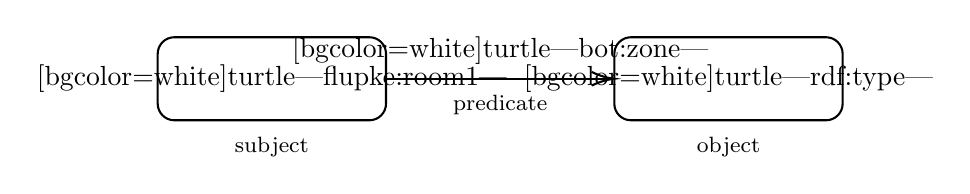
\begin{tikzpicture}[x=0.75pt,y=0.75pt,yscale=-1,xscale=1]
    %uncomment if require: \path (0,300); %set diagram left start at 0, and has height of 300

    %Rounded Rect [id:dp16428191799546488] 
    \draw   (80,68) .. controls (80,63.58) and (83.58,60) .. (88,60) -- (182,60) .. controls (186.42,60) and (190,63.58) .. (190,68) -- (190,92) .. controls (190,96.42) and (186.42,100) .. (182,100) -- (88,100) .. controls (83.58,100) and (80,96.42) .. (80,92) -- cycle ;
    %Rounded Rect [id:dp211253547738401] 
    \draw   (300,68) .. controls (300,63.58) and (303.58,60) .. (308,60) -- (402,60) .. controls (406.42,60) and (410,63.58) .. (410,68) -- (410,92) .. controls (410,96.42) and (406.42,100) .. (402,100) -- (308,100) .. controls (303.58,100) and (300,96.42) .. (300,92) -- cycle ;
    %Straight Lines [id:da3976910390317223] 
    \draw    (190,80) -- (298,80) ;
    \draw [shift={(300,80)}, rotate = 180] [color={rgb, 255:red, 0; green, 0; blue, 0 }  ][line width=0.75]    (10.93,-3.29) .. controls (6.95,-1.4) and (3.31,-0.3) .. (0,0) .. controls (3.31,0.3) and (6.95,1.4) .. (10.93,3.29)   ;

    % Text Node
    \draw (135,80) node   [align=left] {\mintinline[bgcolor=white]{turtle}|flupke:room1|};
    % Text Node
    \draw (355,80) node   [align=left] {\mintinline[bgcolor=white]{turtle}|rdf:type|};
    % Text Node
    \draw (245,66.5) node   [align=left] {\mintinline[bgcolor=white]{turtle}|bot:zone|};
    % Text Node
    \draw (135,113) node  [font=\footnotesize] [align=left] {subject};
    % Text Node
    \draw (355,113) node  [font=\footnotesize] [align=left] {object};
    % Text Node
    \draw (245,92.5) node  [font=\footnotesize] [align=left] {predicate};


\end{tikzpicture}

	\caption{Triple structure}
	\label{fig:triple}
\end{figure}

The basic, yet versatile, structure of a triple is illustrated in Figure \ref{fig:triple}. Both the subject and object are considered as nodes in the data graph, and they are linked by the predicate, which is referred to as an edge. Multiple triples can thus create and link multiple nodes or enrich a connection between two nodes by creating new edges between them. Each element contains a single resource that can be one of the three types: a \acs{uri}, a literal, or a blank node. A \ac{uri} points to a resource on the web and, as its name states, is unique and unambiguous, thus enabling queries and reasoning of the same nature. A literal is a value, and a blank node is an anonymous resource, sometimes used as a placeholder when the exact resource is not known or not necessary to specify. Due to their nature, a subject must be either a \ac{uri} or a blank node, a predicate exclusively a \ac{uri}, and the object may be any of the three types. As \ac{uri} descriptions can be very long, a prefix can be used to shorten them. This is illustrated in Listing \ref{lst:rdfSample} with the \mintinline{turtle}|@prefix bot: <https://w3id.org/bot#>|, which declares that \mintinline{turtle}|bot:Zone| refers, in its full length, to the address \mintinline{turtle}|<https://w3id.org/bot#Zone>|.

This basic concept can be extrapolated to describe and store any kind of data. The advantage for the \ac{aec} industry would be to allow any stakeholders to describe and enrich the knowledge base of a building.

\subsection{Ontologies and reasoning}\label{subsec:ontologies}
When looking at Listing \ref{lst:rdfSample}, a distinction can be made between two types of statements: some refer to classes or properties, such as \mintinline{turtle}|flupke:room1|, while others refer to facts associated with them, like \mintinline{turtle}|rdf:type|. The former is referred to as TBox for \enquote{terminology}, and the latter is referred to as ABox for \enquote{assertions}. The TBox is the part of the ontology that describes the classes and properties of the domain, while the ABox is the part of the ontology that describes the facts about the domain.

By developing an ontology, the domain of interest and the relationships between the classes and properties can be described. This is achieved by defining the classes and properties of the domain and their relationships. The ontology is then used to reason about the domain, inferring new facts based on the ontology and the existing facts within the domain. This is done by a reasoner, which is software capable of performing the reasoning itself on the ontology and associated data. As mentioned, the reasoner can be used to infer new facts, check if created facts are consistent with the ontology, and check if the ontology itself is consistent.\footcite{w3cInfering} It is often integrated with \ac{rdf} databases, also known as triplestores or graph databases.

Classes, properties, and their relationships can be defined using \ac{rdfs}, which is a vocabulary for describing \ac{rdf} schemas using a basic set of constructs. As an extension of \ac{rdfs}, \ac{owl} is a vocabulary for describing ontologies using a more expressive set of constructs tailored to the needs of ontologies. Both \ac{rdfs} and \ac{owl} are considered to be formal ontologies themselves, as they describe the classes and properties of the domain of \ac{rdf}.

\subsection{Triplestores and \acs{sparql}}
As briefly discussed in \ref{subsec:ontologies}, triplestores are \ac{rdf} databases that store data in the form of a graph. They are used to store and query Linked Data and are often integrated with a reasoner. The data itself is retrieved and modified using the \ac{sparql}.\footcite{w3cQuery} In contrast to \ac{sql}, \ac{sparql} queries are able to work across multiple triplestores, called \ac{sparql} endpoints. These are known as federated queries, and their results are combined into a single result set. This is useful when the data is distributed across multiple triplestores in a decentralized manner.\footcite{ontotextSpaql} For example, multiple stakeholders participating in a project, each with their own database.

\subsection{Complexity of the data graph}
The complexity of the data graph is a major concern when working with \ac{ldbim}. This section discusses the origins of the different sources of geometric data that enrich it.

\begin{figure}[h]
	\centering
	% made with Mathcha.io


\tikzset{every picture/.style={line width=0.75pt}} %set default line width to 0.75pt        

\begin{tikzpicture}[x=0.75pt,y=0.75pt,yscale=-1,xscale=1]
%uncomment if require: \path (0,300); %set diagram left start at 0, and has height of 300

%Shape: Polygon [id:ds4126631998252326] 
\draw  [draw opacity=0][fill=ugentblue  ,fill opacity=0.1 ] (450,80) -- (330,110) -- (260,140) -- (190,170) -- (150,200) -- (111,230) -- (190.5,230) -- (330.5,230) -- (450,230) -- cycle ;
%Shape: Axis 2D [id:dp25955824164456476] 
\draw  (70,230) -- (480,230)(111,50) -- (111,250) (473,225) -- (480,230) -- (473,235) (106,57) -- (111,50) -- (116,57)  ;
%Straight Lines [id:da8990032720455088] 
\draw  [dash pattern={on 4.5pt off 4.5pt}]  (150,230) -- (150,200) ;
%Straight Lines [id:da9940965613330952] 
\draw  [dash pattern={on 4.5pt off 4.5pt}]  (190,230) -- (190,170) ;
%Straight Lines [id:da6027058792404336] 
\draw  [dash pattern={on 4.5pt off 4.5pt}]  (260,230) -- (260,140) ;
%Straight Lines [id:da7550073974193503] 
\draw    (105,80) -- (117,80) ;
%Straight Lines [id:da884723975562344] 
\draw    (105,110) -- (117,110) ;
%Straight Lines [id:da05037607471518668] 
\draw    (105,140) -- (117,140) ;
%Straight Lines [id:da007714478926040602] 
\draw    (105,170) -- (117,170) ;
%Straight Lines [id:da9816040608343874] 
\draw    (105,200) -- (117,200) ;
%Straight Lines [id:da025225624633674615] 
\draw [color={rgb, 255:red, 0; green, 0; blue, 0 }  ,draw opacity=0.2 ] [dash pattern={on 0.84pt off 2.51pt}]  (117,80) -- (460,80) ;
%Straight Lines [id:da5278535637091832] 
\draw [color={rgb, 255:red, 0; green, 0; blue, 0 }  ,draw opacity=0.2 ] [dash pattern={on 0.84pt off 2.51pt}]  (117,200) -- (460,200) ;
%Straight Lines [id:da9267646554141478] 
\draw [color={rgb, 255:red, 0; green, 0; blue, 0 }  ,draw opacity=0.2 ] [dash pattern={on 0.84pt off 2.51pt}]  (117,170) -- (460,170) ;
%Straight Lines [id:da7673748768093707] 
\draw [color={rgb, 255:red, 0; green, 0; blue, 0 }  ,draw opacity=0.2 ] [dash pattern={on 0.84pt off 2.51pt}]  (117,140) -- (460,140) ;
%Straight Lines [id:da07336044991653057] 
\draw [color={rgb, 255:red, 0; green, 0; blue, 0 }  ,draw opacity=0.2 ] [dash pattern={on 0.84pt off 2.51pt}]  (117,110) -- (460,110) ;
%Straight Lines [id:da5670615479034977] 
\draw  [dash pattern={on 4.5pt off 4.5pt}]  (330,230) -- (330,110) ;
%Straight Lines [id:da5948760506054469] 
\draw [color=ugentblue  ,draw opacity=1 ]   (450,80) -- (330,110) -- (260,140) -- (190,170) -- (150,200) -- (111,230) ;

% Text Node
\draw (99,195) node [anchor=north east] [inner sep=0.75pt]  [font=\footnotesize] [align=left] {100};
% Text Node
\draw (61,32) node [anchor=north west][inner sep=0.75pt]   [align=left] {\acs{lod}};
% Text Node
\draw (99,165) node [anchor=north east] [inner sep=0.75pt]  [font=\footnotesize] [align=left] {200};
% Text Node
\draw (99,135) node [anchor=north east] [inner sep=0.75pt]  [font=\footnotesize] [align=left] {300};
% Text Node
\draw (99,105) node [anchor=north east] [inner sep=0.75pt]  [font=\footnotesize] [align=left] {400};
% Text Node
\draw (99,75) node [anchor=north east] [inner sep=0.75pt]  [font=\footnotesize] [align=left] {500};
% Text Node
\draw (213.51,135.8) node [anchor=north west][inner sep=0.75pt]  [font=\small,color=ugentblue  ,opacity=1 ,rotate=-336.97] [align=left] {complexity →};
% Text Node
\draw (491,221) node [anchor=north west][inner sep=0.75pt]   [align=left] {time};
% Text Node
\draw (388.64,233.59) node [anchor=north east] [inner sep=0.75pt]  [font=\footnotesize,rotate=-315] [align=left] {use};
% Text Node
\draw (294.29,233.83) node [anchor=north east] [inner sep=0.75pt]  [font=\footnotesize,rotate=-315] [align=left] {as-built};
% Text Node
\draw (171.42,233.82) node [anchor=north east] [inner sep=0.75pt]  [font=\footnotesize,rotate=-315] [align=left] {detailing};
% Text Node
\draw (225.49,233.82) node [anchor=north east] [inner sep=0.75pt]  [font=\footnotesize,rotate=-315] [align=left] {construction};
% Text Node
\draw (138.12,233.58) node [anchor=north east] [inner sep=0.75pt]  [font=\footnotesize,rotate=-315] [align=left] {design};


\end{tikzpicture}

	\vspace{-0.3cm}
	\caption{Evolution of \acs{lod} during the life-cycle of a building. Based upon the Macleamy Curve \parencite{Ilozor2012}}
	\label{fig:bimGraph}
\end{figure}

\subsubsection{\ac{bim} geometry} \label{subsec:bimGeometry}
The 3D model of a building consists of a multitude of sub-models, describing objects for all the different stakeholders participating in the project. Some describe very large objects, and some very small parts. Both can be defined in their most simple and abstract form or have an intricate and complex geometry. For instance, a door can simply be defined as a box, or up to the level of the screw-thread for the hinge system. The level of abstraction is here described as the \ac{lod}, which is most of the time pre-selected for the needs of a \ac{bim} model, and is applied throughout a single model.

As shown in Figure~\ref{fig:bimGraph}, a standard BIM workflow goes through multiple phases, each with their associated model and \ac{lod}. This makes it an important concept in the \ac{aec} industry, as it allows for a very efficient workflow. The modeling step is approached from a top-down perspective, starting with rougher geometries describing the broader ideas of a concept model and evolving to a more refined model for the construction documentation phase. As the last and longest-standing model, a higher \ac{lod} can be used to describe subtle changes in the evolution of a building during the operation phase.



\subsubsection{\acs{ldbim} geometry}
The interconnectivity of semantics can also be applied to geometry descriptions. This could allow the co-existence of multiple \ac{lod}s in a single model database. Besides storing the evolution of a single element's geometry, it enables the linking of the different \ac{lod}s, described in \ref{subsec:bimGeometry}, to each other. Not only that, but extending onto the size of the models described in Table \ref{tab:sizeModels}, already existing \ac{mep}, structural, alongside many other stakeholders' geometry can be added.

\section{Research questions}
\cite{Johansson2015} presented in their paper a new \ac{bim} viewer equipped with the powerful \ac{chc}++. This is a third-generation occlusion culling algorithm developed by \cite{Mattausch2008}, the first being the \ac{chc} \parencite{Bittner2004}, followed by the \ac{nohc} \parencite{Michael2006}. Their conclusion stated that although occlusion culling is very efficient, it is still bound to the scene size, which is limited by hardware capabilities. More precisely, the \ac{gpu}, \ac{vram}, and \ac{ram} capacities.

This thesis proposes the introduction of culling algorithm technology within the context of \ac{ldbim} to address the previously mentioned issue of the scene's size, by culling the scene at its source prior to sending it to the viewer. As culling algorithms have been extensively researched and continue to evolve, as described in the previous paragraph, the research questions in this thesis concentrate on assessing the feasibility of introducing such algorithms in \ac{ldbim}. It aims to propose a set of possible solutions tailored to this specific problem, while highlighting possibilities for future research and specific use cases.

\subsection[Can \acs{ldbim} be culled?]{To what extent can \acs{ldbim} geometry be culled \\
	to be streamed to lightweight viewers?}
This thesis focuses on computing with data snippets or triples inside a \ac{ldbim} model, not within. Meaning that the smallest unit of data that can be culled is the one described in one triple, which is in the most likely scenario, a single \ac{lod} of a single element. It implies that geometry is defined and separated at the object-level. It also implies that culling techniques such as back-face culling will not be handled in this thesis, and will be left to the viewer itself, not the database.

Which snippets of data are needed by the viewer? Is part of the question. The basic needs of the viewer consist firstly of the geometry itself, selecting the right geometry format for the application as well as the additional visual information such as color, texture, etc. Secondly, the identifier of each element is of crucial importance to maintain the link to other semantic resources in the graph. This enables the viewer to retrieve those resources for a multitude of use cases, transforming it into a user-friendly visual query tool.

\subsection[Can existing semantics be used?]{Can existing semantics and ontologies be used\\
	to feed possible culling algorithms?}\label{subsec:rq2}
In contrast to the computer graphics industry, this interconnected context already contains both explicit and implicit, through inferencing, relationships inside the graph. Similarly to \cite{Johansson2009} and their paper where they used the semantics of a \ac{bim} model in \ac{ifc} format to develop culling techniques. However, this thesis will focus on the use of Semantic Web resources. Therefore, it will analyze both \ac{aec}-specific and \ac{aec}-related ontologies, such as \ac{gis}-related, to see if they can be used to feed culling algorithms.